%*******10********20********30********40********50********60********70********80

% For all chapters, use the new defined chap{} instead of chapter{}
% This will make the text at the top-left of the page be the same as the chapter

\chap{Method of Simulation Models}

\section{Rigid Body Spring Model (RBSM)}

The simulations are carried out by the three dimensional RBSM, proposed by Kawai \textit{et al}.(1978). By using 3D RBSM, a concrete model is meshed into rigid bodies, with each consists six degree of freedoms, shown in \textbf{fig.}.

fig

These six freedoms are three transitional freedoms and three rotational freedoms at the center point within the element.

The computational point $(x_c, y_c, z_c)$ is defined as,

\begin{equation}
  \begin{aligned}
  &x_c=\frac{x_1 + x_2 + \cdots + x_i + \cdots + x_m}{m} \\
  &y_c=\frac{y_1 + y_2 + \cdots + y_i + \cdots + y_m}{m} \\
  &z_c=\frac{z_1 + z_2 + \cdots + z_i + \cdots + z_m}{m}
  \end{aligned}
\end{equation}

where m is the number of node composing an element and $x_i$, $y_i$ and $z_i$ are the coordinates of the nodes in an element.

Three individual springs, which are one normal spring and two shear spring, are set at a point on the face between two elements. This point $(x_{cf}, y_{cf}, z_{cf})$ is defined as,

\begin{equation}
  \begin{aligned}
  &x_{cf}=\frac{x_1 + x_2 + \cdots + x_j + \cdots + x_n}{n} \\
  &y_{cf}=\frac{y_1 + y_2 + \cdots + y_j + \cdots + y_n}{n} \\
  &z_{cf}=\frac{z_1 + z_2 + \cdots + z_j + \cdots + z_n}{n}
  \end{aligned}
\end{equation}

Where m is the number of nodes composing the face and $x_j$, $y_j$ and $z_j$ are those coordinates.

Since cracks initiate and propagate along the boundary face, the mesh arrangement may affect fracture direction. Random geometry is introduced to avoid the formation of cracks in a certain direction by using a Voronoi diagram
\textbf{figure}.

In the nonlinear analysis, a stiffness matrix is constructed based on the principle of virtual work (Kawai and Takeuchi 1990), and the Modified Newton-Raphson method is employed for the convergence algorithm.

When an element has small displacement $[u_1, v_1, w_1, \theta_{u1}, \theta_{v1}, \theta_{w1}]$, the springs at a face in an element will be displaced:

\begin{equation}
  \begin{aligned}
  &u = u_1 - \theta_{w1} (y_{cf} - y_{ce1}) + \theta_{v1} (z_{cf} - z_{ce1}) \\
  &v = v_1 - \theta_{u1} (z_{cf} - z_{ce1}) + \theta_{w1} (x_{cf} - x_{ce1}) \\
  &w = w_1 - \theta_{v1} (x_{cf} - x_{ce1}) + \theta_{u1} (y_{cf} - y_{ce1})
  \end{aligned}
\end{equation}

Elongations of normal and shear spring are calculated and expressed as:

\begin{equation}
  d = Bu_e
\end{equation}

where $d^T = [\delta_{s1}, \delta_{s2}, \delta_n]$ and $u_e^T = [u_1, v_1, w_1,\theta_{u1}, \theta_{v1}, \theta_{w1}, u_2, v_2, w_2,\theta_{u2}, \theta_{v2}, \theta_{w2}]$

The transformation matrix B is written as:

\begin{equation}
  B =
  \begin{vmatrix}
    K_{11} &K_{12} &K_{13} &K_{14} &{\cdots} &K_{19} &K_{110} &K_{111} &K_{112}\\
    K_{21} &K_{22} &K_{23} &K_{24} &{\cdots} &K_{29} &K_{210} &K_{211} &K_{212}\\
    K_{31} &K_{32} &K_{33} &K_{34} &{\cdots} &K_{39} &K_{310} &K_{311} &K_{312}
  \end{vmatrix}
\end{equation}

where \\
$K_{11} = -e_{s1x}$    $K_{21} = -e_{s2x}$    $K_{31} = -e_{nx}$ \\
$K_{12} = -e_{s1y}$    $K_{22} = -e_{s1y}$    $K_{32} = -e_{ny}$ \\
$K_{13} = -e_{s1z}$    $K_{23} = -e_{s2z}$    $K_{33} = -e_{nz}$ \\
\\
$K_{14} = e_{s1y}(z_{cf}-z{ce1})-e_{s1z}(y_{cf}-y_{ce1})$\\
$K_{24} = e_{s2y}(z_{cf}-z{ce1})-e_{s2z}(y_{cf}-y_{ce1})$\\
$K_{34} = e_{ny}(z_{cf}-z{ce1})-e_{nz}(y_{cf}-y_{ce1})$\\
\\
$K_{15} = e_{s1z}(x_{cf}-x{ce1})-e_{s1x}(z_{cf}-z_{ce1})$\\
$K_{25} = e_{s2z}(x_{cf}-x{ce1})-e_{s2x}(z_{cf}-z_{ce1})$\\
$K_{35} = e_{nz}(x_{cf}-x{ce1})-e_{nx}(z_{cf}-z_{ce1})$\\
\\
$K_{15} = e_{s1z}(x_{cf}-x{ce1})-e_{s1x}(z_{cf}-z_{ce1})$\\
$K_{25} = e_{s2z}(x_{cf}-x{ce1})-e_{s2x}(z_{cf}-z_{ce1})$\\
$K_{35} = e_{nz}(x_{cf}-x{ce1})-e_{nx}(z_{cf}-z_{ce1})$\\
\\
$K_{16} = e_{s1x}(y_{cf}-y{ce1})-e_{s1y}(x_{cf}-x_{ce1})$\\
$K_{26} = e_{s2x}(y_{cf}-y{ce1})-e_{s2y}(x_{cf}-x_{ce1})$\\
$K_{36} = e_{nx}(y_{cf}-y{ce1})-e_{ny}(x_{cf}-x_{ce1})$\\
\\
$K_{17} = e_{s1x}$    $K_{27} = e_{s2x}$    $K_{37} = e_{nx}$ \\
$K_{18} = e_{s1y}$    $K_{28} = e_{s1y}$    $K_{38} = e_{ny}$ \\
$K_{19} = e_{s1z}$    $K_{29} = e_{s2z}$    $K_{39} = e_{nz}$ \\
\\
$K_{110} = e_{s1z}(y_{cf}-y{ce2})-e_{s1y}(z_{cf}-z_{ce2})$\\
$K_{210} = e_{s2z}(y_{cf}-y{ce2})-e_{s2y}(z_{cf}-z_{ce2})$\\
$K_{310} = e_{nz}(y_{cf}-y{ce2})-e_{ny}(z_{cf}-z_{ce2})$\\
\\
$K_{111} = e_{s1x}(z_{cf}-z{ce2})-e_{s1z}(x_{cf}-x_{ce2})$\\
$K_{211} = e_{s2x}(z_{cf}-z{ce2})-e_{s2z}(x_{cf}-x_{ce2})$\\
$K_{311} = e_{nx}(z_{cf}-z{ce2})-e_{nz}(x_{cf}-x_{ce2})$\\
\\
$K_{112} = e_{s1y}(x_{cf}-x{ce2})-e_{s1x}(y_{cf}-y_{ce2})$\\
$K_{212} = e_{s2y}(x_{cf}-x{ce2})-e_{s2x}(y_{cf}-y_{ce2})$\\
$K_{312} = e_{ny}(x_{cf}-x{ce2})-e_{nx}(y_{cf}-y_{ce2})$\\

where $e_{ij}$ is direction cosine in i axis on j axis.

By applying the principal of virtual work, the local equilibrium relation expressed in global coordinate is:

\begin{equation}
  k_e \delta u_e = \delta f_e
\end{equation}

where the stiffness associated with interconnected face $k_e$ is given as:

\begin{equation}
  k_e = B^T DB
\end{equation}

where
\begin{equation}
  D = \begin{vmatrix}
        k_{s1} &0 &0 \\
        0 &k_{s2} &0 \\
        0 &0 &k_3
      \end{vmatrix}
\end{equation}

in which $k_n$, $k_{s1}$, and $k_{s2}$ are the normal and shear spring stiffness. $k_n$, $k_{s1}$, and $k_{s2}$ can be calculated as:
\begin{equation}
  \begin{aligned}
    &k_n = k_{sp} \frac{A}{h_1 + h_2} \\
    &k_{s1} = k_{ssp} \frac{A}{h_1 + h_2} \\
    &k_{s2} = k_{ssp} \frac{A}{h_1 + h_2}
  \end{aligned}
\end{equation}

where

\begin{equation}
  \begin{aligned}
    &k_{nsp} = \frac{(1-\theta_{elem})E_{elem}}{(1+\theta_{elem})(1-2\theta_{elem})} \\
    &k_{ssp} = \frac{E_{elem}}{1+\theta_{elem}}
  \end{aligned}
\end{equation}

where $h_1$ and $h_2$ are length of perpendicular lines from the element computational point to the face where springs are set.

$E_{elem}$ and $v_{elem}$ are the modulus of elasticity and poison's ratio, respectively:

\begin{equation}
  \begin{aligned}
    &E_{elem} = \frac{E_{elem1} h_1 + {E_{elem2} h_2}}{h_1+h_2} \\
    &\theta_{elem} = \frac{\theta_{elem1} h_1 + {\theta_{elem2} h_2}}{h_1+h_2}
  \end{aligned}
\end{equation}

In the convergence process, displacements that cancel the unbalanced force of elements are added to the elements.

The displacements are calculated using the stiffness matrix. Convergence of the model is judged when the ratio of
$\sum_{} $(Unbalanced force of element in the model)$^2$ to \\
$\sum_{} $(Applied force to element)$^2$ becomes less than $10^5$.
%*******10********20********30********40********50********60********70********80

\section{Constitutive Model}

\subsection{Mortar Model}

In this study, constitutive model for concrete at meso scale is developed because constitutive model at the  macro scale cannot be applied directly to meso scale analysis.

The material characteristics of each component are presented by means of modeling spring.

PIC Constitutive models of concrete

In normal springs, compressive and tensile stresses ($\theta$) are developed. Shear springs develop shear stress ($\tau$). The elastic modulus of normal spring ($k_n$) and shear spring ($k_s$) are presented assuming a plane strain condition, where kn and ks are the elastic modulus of normal and shear spring, and $E_{elem}$ and $v_{elem}$ are the corrected elastic modulus and Poisson’s ratio of component at the meso scale, respectively.

\begin{equation}
  \begin{aligned}
   &\theta_{elem} = -24.8\theta^4 + 31.9\theta^3 - 16.4\theta^2 + 4.28\theta \\
   &E_{elem} = (-33.7\theta_{elem}^4 + 17.0\theta_{elem}^3 - 4.13\theta^2 + 0.327\theta_{elem}+1)E
  \end{aligned}
\end{equation}

For calculation of shear stress, a resultant value of strains generated in two shear springs is adopted as a shear strain in the constitutive model presented in this chapter.

\begin{equation}
  \begin{aligned}
   &\varepsilon = \frac{\delta_n}{h_1+h_2} \\
   &\gamma = \frac{\delta_s}{h_1+h_2} \\
   &\sigma = k_{nsp}\varepsilon \\
   &\tau = k_{ssp}\gamma
  \end{aligned}
\end{equation}

\subsection{Aggregate Model}

In this study, the effect of the existence of aggregate in
concrete on the fracture process is examined. For this
purpose, aggregate elements are assumed to behave only
elastically without fracture in this study.

The same equations as (3?), (4?), (5?) and (7?) are adopted to present the material property of aggregate.

Pic Of AGGREGATE

\subsection{Expansion Model}

In the expansive behavior of DEF and ASR, the expanse is caused by strains generated from within the concrete when there is no external loading.

One of the similar behavior in previous research is the strength development due to autogenous shrinkage in high strength concrete, which was carried out by Osakabe et al. (2014). The concept of initial strain in RBSM has been successfully utilized in the simulation of the behavior of autogenous shrinkage in high strength concrete.

The same concept of initial strain is utilized in the present of ASR and DEF expanse behavior carried out by L.EDDY et al. in 2016. Characteristic map cracking pattern in ASR simulation was presented successfully, while the DEF simulation results do not match well with the typical map cracking pattern observed in the real concrete.

The concept of the initial strain used in this simulation is based on the case where a specimen expansion occurs without any constraint.

Fig

P99 Left

According to  3D RBSM developed by Nagai et al. (2005), the first step is the calculation of actual force, which supposed to be calculated by solving strain, stress and force matrices of all elements in sequence based on input data and boundary condition.

Iteration is then performend until this force under the acceptable limit with an external force. When the convergence condition is reached, the same sequence will be performed for the next step.

In our simulation, one additional step of introducing the initial strain is added here to simulate the behavior of expansion.  Then, Stresses due to this initial strain are calculated in the next step, with considering the initial strain added. After the stress is calculated, the initial strain added up earlier will be subtracted, before the forces are calculated.

The illustration of introducing initial strain is shown in the Fig \ref.
Fig P101

For ASR and DEF, the initial strains are introduced at different interfaces in concrete.

Expansion is giving to simulative the behavior of model up to 1.3\% expansion(in one dimensional).

Fig. illustration of one-dimensional expansion.

\subsubsection{ASR Expansion Behavior In Simulation}

For ASR expansion, the expanse is generated at the location of interfaces between mortar and aggregate. The concept of the initial strain is used here to introduce the expansion.

Fig. illustration

As we consider the ratio of reactive aggregate may differ the behavior of the model in ASR expansion,  cases of different percentage aggregate expanse are simulated and cross-compared. The reactive aggregates are also chosen randomly.

Fig P128

As in the research done by L.EDDY et al. (2016), the desired characteristic map cracking pattern of ASR expansion has already achieved in this method. In this simulation, the discussion is focused on the relationship between cracking pattern with aggregate percentage, reactive aggregate, expanding ratio, also the residual mechanical properties of ASR-damaged concrete.

\subsubsection{DEF Expansion Behavior In Simulation}

Similar model and mechanism are also applied in the simulation of DEF  type expansion. Following the popular theory of expansion in DEF  is caused by expansion of paste, initial strain here is given to the interfaces between mortar elements to present the DEF expansion.

According to the previous study done by L.EDDY et al, simple uniformed paste expansion theory need improvement. Whether for cases giving initial strain to 100\%, 50\% or 25\% random faces of mortar chosen to expanse, the surface of expanded concrete does not match with the actual cracking pattern.

It is well established that high early temperature experienced by the concrete is the most important factor inducing DEF in concrete. (Ghorab et al (1980), Ludwig(1987), Sylla(1988), Hanehara \& Oyamada(2010), Rasiah and Stephen(2014) etc.)

The research done by Anupam (2016) confirmed the rising of the temperature inside concrete due to combination effect of steam curing and heat of hydration inside the concrete is not uniform. Both the simulation result is done by Astea Macs (FEM based non-linear thermal stress analysis program developed by Research Center of Computational Mechanics, Japan) and the field measurement of temperature rising process inside concrete during steam curing in a concrete plant located in India shows the un-uniformed distribution of maximum temperature experienced. The temperature in the center of the concrete structure is significantly higher than the outer part.

Fig P80

The cracking pattern in DEF damaged concrete, recorded by Anupam (2016), also suggested the possibility of non-uniformed expansion happens in DEF damaged concrete structure. The cracking concentrated in the outer part of the structure, while the inner part remained undamaged, showing the trend of larger expansion happening in the inner part of the concrete paste.

Fig

Considering the effect of temperature on triggering  DEF expansion and its characteristic cracking pattern, for DEF simulation, uniform expansion does not quite fit with the real situation. The expansion inside concrete structure supposes to be much severe than the outer part. For which here in this research non-uniformed expanding is introduced by giving a different amount of DEF initial strain considering the location of element.


The inner part of the model will be giving larger initial strain,  present the higher maximum temperature experienced, while the outer part mortar will be giving small or none initial strain.

Fig illustration


\subsection{Conclusions}

In this chapter describe about the numerical simulation system that has been used in this research, RBSM. In the this study, RBSM is used to simulate the deterioration of concrete due to expansion such as expansion crack, then the mechanical properties of expanded concrete will be calculated by using RBSM.

In RBSM, the response of normal spring and shear spring represent the mechanical response of mortar and aggregate member. By giving initial strain, the response of spring changed in the relatively close manner as real expanded structure. The details of simulation results from this simulation will be described again in Chapter 4.



%*******10********20********30********40********50********60********70********80

\section{Details of Numerical Models for ASR Simulation}

\subsection{Geometry of Numerical Models}

Figure X shows the geometry of the model, which is in dimension of 100 x 100 x 100mm. Numbers of elements varies from XXXXX to XXXXX. Average diameter of meshed element is around 2mm.

\subsection{Coarse Aggregate of Numerical Models}

To analysis the behavior of concrete with different coarse aggregate volume ratio, 15\% coarse aggregate model(Fig.X) and 30\% coarse aggregate model(Fig.X) are built for simulation.

\begin{figure}[ht!]
\centering
\begin{subfigure}{.5\textwidth}
  \centering
  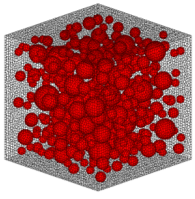
\includegraphics[width=.4\linewidth]{Files/Aggregate/A15.png}
  \caption{15\% Coarse Aggregate}
  \label{fig:A15_model}
\end{subfigure}%
\begin{subfigure}{.5\textwidth}
  \centering
  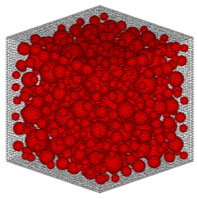
\includegraphics[width=.4\linewidth]{Files/Aggregate/A30.png}
  \caption{30\% Coarse Aggregate}
  \label{fig:A30_model}
\end{subfigure}
\caption{Coarse Aggregate Percentage}
\label{fig:Aggregate_Percentage}
\end{figure}

\subsection{ASR Reactive Coarse Aggregate Ratio}

To analysis the behavior of concrete with different ASR reactive coarse aggregate ratio, 25\% ASR reactive coarse aggregate ratio model and 25\% ASR reactive coarse aggregate ratio model are built for 30\% aggregate case.

\begin{figure}[!h]
\centering
\begin{subfigure}{.5\textwidth}
  \centering
  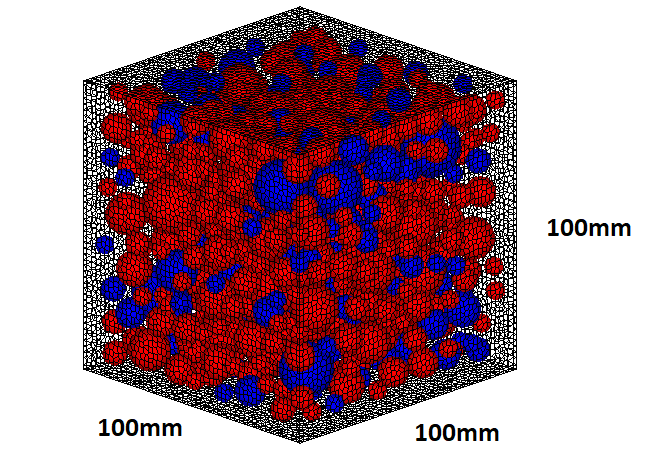
\includegraphics[width=.8\linewidth]{Files/Aggregate/A30P75.png}%FIXME
  \caption{30\% Coarse Aggregate with 75\% ASR Reactive Aggregate}
\end{subfigure}%
\begin{subfigure}{.5\textwidth}
  \centering
  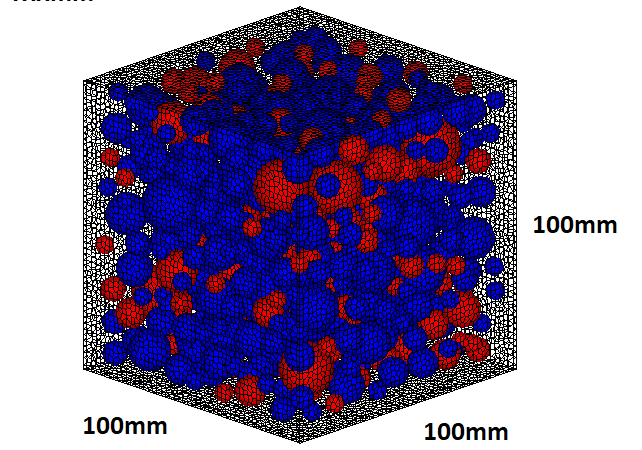
\includegraphics[width=.8\linewidth]{Files/Aggregate/A30P25.png} %FIXME
  \caption{30\% Coarse Aggregate with 25\% ASR Reactive Aggregate}
\end{subfigure}
\caption{25\% and 75\% ASR Reactive Aggregate Ratio Model}
\label{fig:Aggregate_Percentage}
\end{figure}

\subsection{Boundary Conditions}

\subsubsection{Boundary Condition During ASR Expansion}

During ASR Expansion, no confinements are added to the boundary elements. Models expanse freely in all directions.

\subsubsection{Boundary Conditions During Uni-axial Loading Test}

Fig X and X show the boundary condition of simulation models for uni-axial loading test.

fig

In the case of fixed boundary condition, displacement in all directions are assumed as 0 at the bottom. Displacement in horizontal directions are all assumed as 0 at the top, and displacement in vertical direction is increased by 0.02mm downward at each loading step.

fig

In the case of free boundary condition, all boundary elements able to move freely in horizontal direction except 2 center elements in top and bottom are fixed in horizontal direction, to prevent the sliding of whole model during loading. Same as fixed boundary condition cases, displacement in vertical direction is increased by 0.02mm downward at each loading step for top boundary elements.

Loading is applied until the maximum compressive strength is reached.

\subsection{Initial Strain Given For ASR Expansion}

To analysis the relationship of concrete behavior and mechanical properties with expansion amount, initial strain is given between reactive aggregate and mortar.

\begin{table}[ht!]
\centering
\begin{tabular}{ ||p{2cm}|p{2cm}|p{2cm}|p{2cm}|p{2cm}|| }
 \hline
 Aggregate Ratio[\%] &  Reactive Aggregate Ratio[\%] & Boundary Condition & Initial Strain (Each Step) & Expanding Steps \\ [0.5ex]
 \hline\hline
 15 & 11.25 & Fix & 0 & 0 \\
 15 & 11.25 & Fix & 0.0002 & 20 \\
 15 & 11.25 & Fix & 0.0005 & 20 \\
 15 & 11.25 & Fix & 0.001 & 20 \\
 15 & 11.25 & Fix & 0.002 & 20 \\
 15 & 11.25 & Fix & 0.003 & 20 \\

 15 & 11.25 & Free & 0 & 0 \\
 15 & 11.25 & Free & 0.0002 & 20 \\
 15 & 11.25 & Free & 0.0005 & 20 \\
 15 & 11.25 & Free & 0.001 & 20 \\
 15 & 11.25 & Free & 0.002 & 20 \\

 30 & 22.50 & Fix & 0 & 0 \\
 30 & 22.50 & Fix & 0.0002 & 20 \\
 30 & 22.50 & Fix & 0.0005 & 20 \\
 30 & 22.50 & Fix & 0.001 & 20 \\
 30 & 22.50 & Fix & 0.002 & 20 \\
 30 & 22.50 & Fix & 0.003 & 20 \\

 30 & 22.50 & Free & 0 & 0 \\
 30 & 22.50 & Free & 0.0002 & 20 \\
 30 & 22.50 & Free & 0.0005 & 20 \\
 30 & 22.50 & Free & 0.001 & 20 \\
 30 & 22.50 & Free & 0.002 & 20 \\

 30 & 7.50 & Fix & 0 & 0 \\
 30 & 7.50 & Fix & 0.001 & 20 \\
 30 & 7.50 & Fix & 0.002 & 20 \\
 30 & 7.50 & Fix & 0.004 & 20 \\
 30 & 7.50 & Fix & 0.006 & 20 \\  [0.5ex]
 \hline
\end{tabular}
\caption{ASR Models}
\label{table:ASR_MODELS}
\end{table}

%*******10********20********30********40********50********60********70********80

\section{Details of Numerical Models for DEF Simulation}

\subsection{Introduction}

The exactly same model is used for DEF simulation in order to cross compare the cracking patterns and mechanical properties changes under ASR and DEF expansion.

\subsection{Geometry of Numerical Models}

The geometry of the models is exactly the same as models using in ASR simulation, which is in dimension of 100 x 100 x 100mm.

All materials properties are set to be exactly the same.

\subsection{Coarse Aggregate of Numerical Models}

To analysis the behavior of concrete with different coarse aggregate volume ratio, 15\% coarse aggregate model(Fig.X) and 30\% coarse aggregate model(Fig.X) are built for simulation.

\subsection{DEF Intensified Expansion Area of Numerical Models}

Since DEF is closely related to higher curing temperature, here we choose to intensified the expansion in center part of model.

Here we chooses 3 cases in different expansion intensified area. The \textbf{table \ref{table:DEF_X}} is a list of cases simulated.

\begin{table}[ht!]
\centering
\begin{tabular}{||c c c||}
 \hline
 Case &  Expansion Intensified Depth[mm] &  Expansion Intensified Area[\%] \\ [0.5ex]
 \hline\hline
 1 & 0 & 100 \\
 2 & 12.5 & 56.25 \\
 3 & 25 & 25 \\ [0.5ex]
 \hline
\end{tabular}
\caption{DEF Intensified Expansion Area}
\label{table:DEF_X}
\end{table}

\begin{figure}[ht]
\centering
    %*******
    \begin{subfigure}{.33\textwidth}
      \centering
      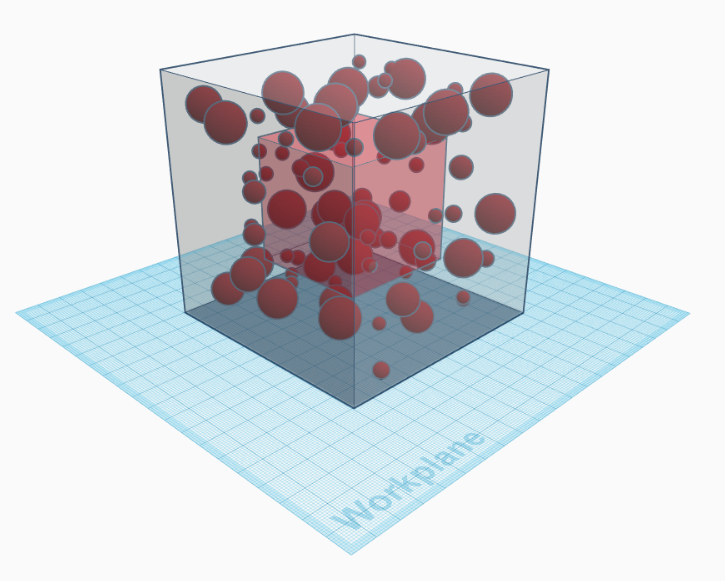
\includegraphics[width=.8\linewidth]{Files/DEF_X/X0_3d.png}
      \caption{Intensified  \\ 50x50x50mm Case}
    \end{subfigure}%
    %*******
    \begin{subfigure}{.33\textwidth}
      \centering
      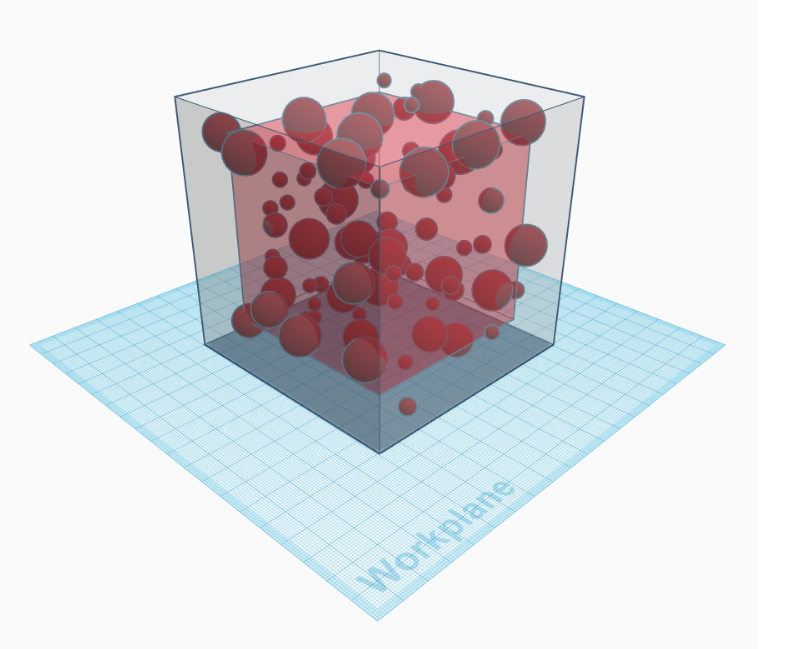
\includegraphics[width=.8\linewidth]{Files/DEF_X/X-5_3d.png}
      \caption{Intensified  \\ 75x75x75mm Case}
    \end{subfigure}%
    %*******
    \begin{subfigure}{.33\textwidth}
      \centering
      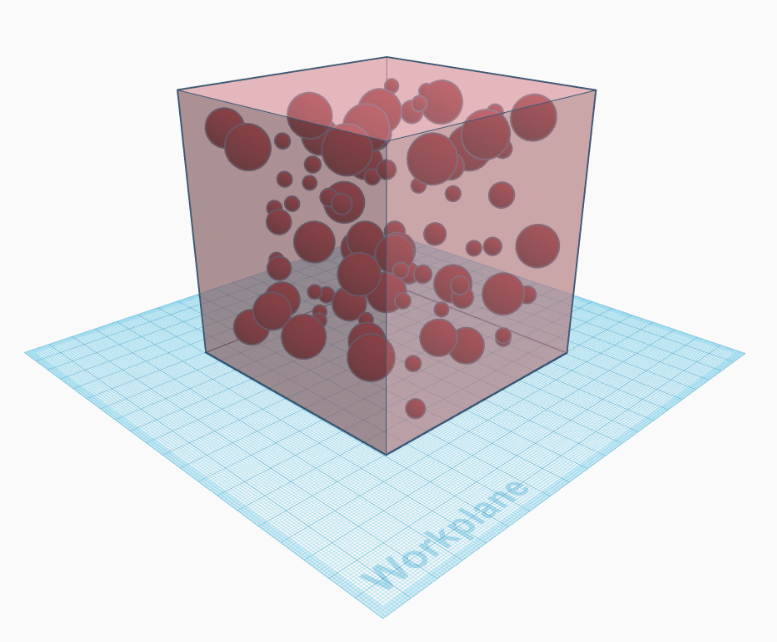
\includegraphics[width=.8\linewidth]{Files/DEF_X/X-1_3d.png}
      \caption{Intensified  \\ 100x100x100mm Case}
    \end{subfigure}
    %*******
    %*******
    \begin{subfigure}{.33\textwidth}
      \centering
      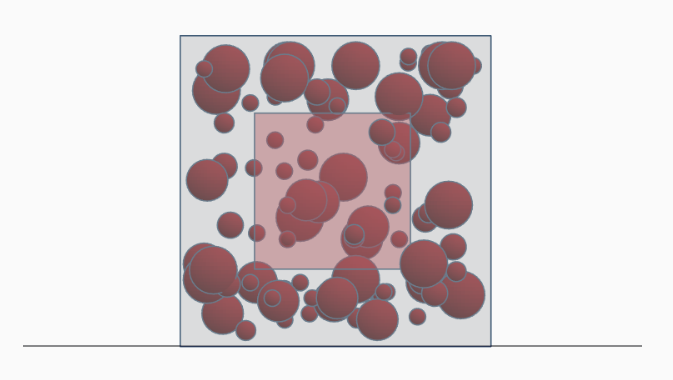
\includegraphics[width=.8\linewidth]{Files/DEF_X/X0_3ds.png}
      \caption{Intensified  \\ 50x50x50mm Case\\ Cross Section}
    \end{subfigure}%
    %*******
    \begin{subfigure}{.33\textwidth}
      \centering
      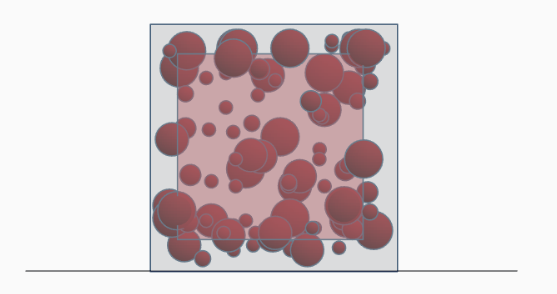
\includegraphics[width=.8\linewidth]{Files/DEF_X/X-5_3ds.png}
      \caption{Intensified \\  75x75x75mm Case \\ Cross Section}
    \end{subfigure}%
    %*******
    \begin{subfigure}{.33\textwidth}
      \centering
      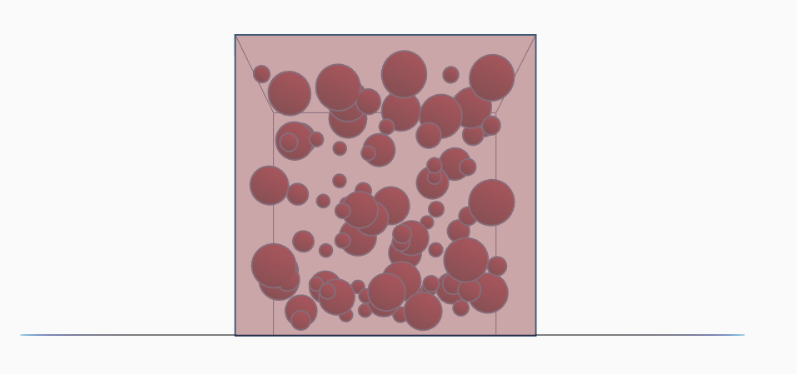
\includegraphics[width=.9\linewidth]{Files/DEF_X/X-1_3ds.png}
      \caption{Intensified  \\ 100x100x100mm Case\\ Cross Section}
    \end{subfigure}
    %*******
  \caption{DEF intensified part range}
  \label{fig:DEF_X}
\end{figure}

\subsection{Boundary Conditions}

\subsubsection{Boundary Condition During DEF Expansion}

Same as in ASR expansion, during DEF expansion, no confinements are added to the boundary elements. Models expanse freely in all directions.

\subsubsection{Boundary Conditions During Uni-axial Loading Test}

Same as in ASR expansion, Uni-axial Loading Test is applied with both fixed and free boundary conditions.

fig

In the case of fixed boundary condition, displacement in all directions are assumed as 0 at the bottom. Displacement in horizontal directions are all assumed as 0 at the top, and displacement in vertical direction is increased by 0.02mm downward at each loading step.

fig

In the case of free boundary condition, all boundary elements able to move freely in horizontal direction except 2 center elements in top and bottom are fixed in horizontal direction, to prevent the sliding of whole model during loading. Same as fixed boundary condition cases, displacement in vertical direction is increased by 0.02mm downward at each loading step for top boundary elements.

Loading is applied until the maximum compressive strength is reached.
